\documentclass{article}
\usepackage{amsmath}   % for mathematical equations
\usepackage{graphicx}  % for including graphs and images
\usepackage{float}     % to force figure placement
\usepackage{caption}   % for figure captions
\usepackage{siunitx}   % for units formatting
\usepackage{hyperref}  % for links

\title{Lab Report IV: Digital Logic}
\author{Enrique Rivera \\ Lab Partner: Marcus}
\date{\today}

\begin{document}
\maketitle

\section*{Lab 10: Digital Circuits I}

    \subsection*{Objective}
    The objective of Lab 10 was to familiarize students with basic logic gates and combinational circuits. The main focus was on building simple logic circuits using AND, OR, and NAND gates and verifying their truth tables through practical implementation.

    \subsection*{\textbf{Procedure - Question 1}}
    In this part of the lab, we used both TTL (7400N or 74LS00N) and CMOS (74HCT00N) ICs to implement individual logic gates. Each IC contains multiple NAND gates that can be configured into other basic gates (AND and OR) by connecting the gates in specific ways.

    \textbf{1. Power Supply Setup:}
    - We set the power supply (Vcc) to 5.04V, which is within the recommended operating range for both TTL and CMOS ICs.
    \\
    - Ground (GND) was connected to the ground terminal on the breadboard, and Vcc was applied to the power pins on the ICs.
    \\

    \textbf{2. Connecting the ICs:}
    - For each IC (TTL and CMOS), we connected Vcc (5.04V) to the designated power pin and ground to the ground pin of the ICs.
    \\
    - All unused inputs were grounded to prevent floating states, as floating inputs can lead to unpredictable behavior in CMOS and TTL logic gates.
    \\

    \textbf{3. Setting Up Inputs with SPDT Switches:}
    - We used SPDT (Single Pole Double Throw) switches on the breadboard to control the inputs for each gate. These switches allowed us to easily switch between 0 (ground) and 1 (Vcc) for each input, enabling us to test all possible input combinations.
    \\

    \textbf{4. Constructing NAND Gate Circuit:}
    - To test the NAND gate, we used one of the gates in the 7400N and 74HCT00N ICs. The input pins were connected to the SPDT switches for A and B, allowing us to manually control the input combinations (0 or 1).
    \\
    - LEDs were connected to the output pin through a current-limiting resistor to visualize the output. A high output (1) would turn the LED on, while a low output (0) would turn the LED off.
    \\

    \textbf{5. Testing Procedure:}
    - We applied all possible combinations of inputs (A and B) using the SPDT switches to observe the output.
    \\
    - For each combination, we recorded the LED state and documented whether the output matched the expected truth table values.
    \\

    \textbf{6. Verification with Multiple Gates:}
    - We repeated the procedure for additional gates on each IC to verify consistency in behavior. This was done by connecting different gate sections of the same IC, setting up inputs in a similar fashion, and observing the output with the same method.
    \\
    - We compared results between the TTL (7400N) and CMOS (74HCT00N) gates to observe any differences in behavior or performance.
    \\


    \subsection*{\textbf{Results - Question 1}}
    The following table and graph illustrate the expected truth table for the NAND gate tested in this question:

    \begin{table}[H]
        \centering
        \caption{Truth Table for NAND Gate}
        \begin{tabular}{|c|c|c|}
            \hline
            Input A & Input B & NAND Output \\
            \hline
            0 & 0 & 1 \\
            0 & 1 & 1 \\
            1 & 0 & 1 \\
            1 & 1 & 0 \\
            \hline
        \end{tabular}
    \end{table}

    \begin{figure}[H]
        \centering
        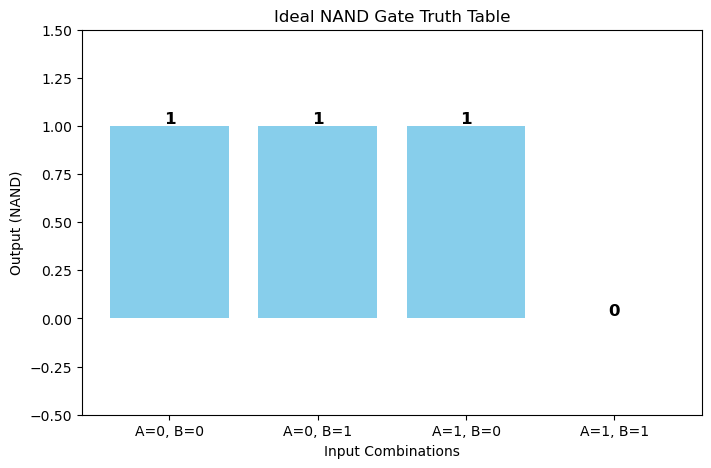
\includegraphics[width=0.7\textwidth]{./img/Lab 10/10_1_1.png}
        \caption{Ideal NAND Gate Truth Table Visualization}
        \label{fig:nand_truth_table}
    \end{figure}

    \subsection*{\textbf{Question 1 - Discussion}}
    The results confirmed that the NAND gate produces an output of 1 for all input combinations except when both inputs are 1, where it outputs 0. This behavior was consistent across both the TTL (7400N) and CMOS (74HCT00N) ICs, demonstrating their reliability in performing NAND operations. The truth table and visualization in Figure \ref{fig:nand_truth_table} match the theoretical expectations, validating the functionality of the NAND gates in our circuit. Additionally, grounding all unused inputs ensured stable outputs, particularly for the CMOS IC, which is more susceptible to interference from floating inputs. 
    \subsection*{\textbf{Procedure - Question 2}}
    In Question 2, we expanded the NAND gate circuit to implement a clocked flip-flop using two additional NAND gates. This configuration allowed us to create a clocked RS (Reset-Set) flip-flop, where the output changes state only when the clock is active.

    \textbf{1. Circuit Setup:}
   - We used the TTL (7400N) and CMOS (74HCT00N) ICs to build the flip-flop circuit.
   \\
   - Vcc was set to 5.04V, and all unused inputs were grounded to prevent floating states.
   \\
   - The circuit was connected so that two additional NAND gates were used to introduce a clock input, along with the S (Set) and R (Reset) inputs.
    \\

   \subsection*{\textbf{Procedure - Question 2}}
   In Question 2, we used multiple NAND gates to construct an \textbf{AND gate}. By configuring NAND gates in a specific arrangement, we replicated the behavior of a standard AND gate.

   \textbf{1. Circuit Setup:}
      - We used the TTL (7400N) and CMOS (74HCT00N) ICs, each containing multiple NAND gates.
      \\
      - Vcc was set to 5.04V, and all unused inputs were grounded to prevent floating states.
      \\
      - To create an AND gate using NAND gates, we connected two NAND gates in series:
      \\
        - The inputs (A and B) were connected to the first NAND gate.
        \\
        - The output of the first NAND gate was connected to both inputs of the second NAND gate (essentially inverting the output of the first NAND gate).
        \\
   
   \textbf{2. Input Control with SPDT Switches:}
      - SPDT switches on the breadboard were used to control the A and B inputs, allowing us to toggle each input between 0 (ground) and 1 (Vcc).
      \\
      - LEDs were used to indicate the output state.
      \\
   
   \textbf{3. Testing Procedure:}
      - We applied all possible combinations of A and B inputs using the SPDT switches and observed the output.
      \\
      - The output state was recorded for each combination to confirm that the NAND gate arrangement produced the expected AND gate behavior.
      \\
   
   \subsection*{\textbf{Results - Question 2}}
   The table below summarizes the expected truth table for the constructed AND gate:
   
   \begin{table}[H]
       \centering
       \caption{Truth Table for AND Gate Constructed with NAND Gates}
       \begin{tabular}{|c|c|c|}
           \hline
           Input A & Input B & AND Output \\
           \hline
           0 & 0 & 0 \\
           0 & 1 & 0 \\
           1 & 0 & 0 \\
           1 & 1 & 1 \\
           \hline
       \end{tabular}
   \end{table}

   \begin{figure}[H]
        \centering
        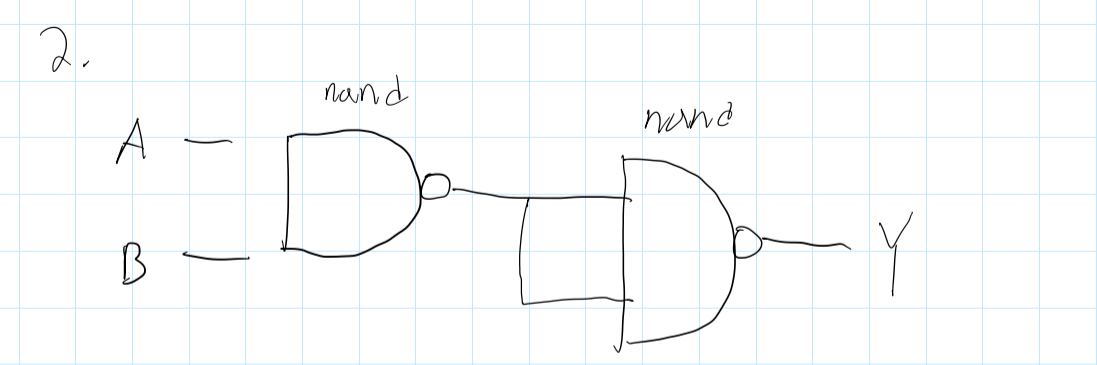
\includegraphics[width=0.7\textwidth]{./img/Lab 10/10_2_1.png}
        \caption{NANDS Gates to Construct AND Gate}
        \label{fig:and_gate}
    \end{figure}
   
   \subsection*{\textbf{Question 2 - Discussion}}
   The results confirmed that the arrangement of NAND gates successfully produced an AND gate. The output matched the expected truth table for an AND gate, outputting 1 only when both inputs were 1. This demonstrates that NAND gates can be used to create other basic gates, such as AND.
   
   \subsection*{\textbf{Procedure - Question 3}}
   In Question 3, we used multiple NAND gates to construct an \textbf{OR gate}. This required additional configuration, as NAND gates inherently perform a different operation.
   
   \textbf{1. Circuit Setup:}
      - We used the TTL (7400N) and CMOS (74HCT00N) ICs to build the OR gate circuit with NAND gates.
      \\
      - Vcc was set to 5.04V, and all unused inputs were grounded.
      \\
      - To create an OR gate using NAND gates, we used three NAND gates as follows:
      \\
        - The inputs A and B were each inverted by connecting them to separate NAND gates (where each input was connected to both pins of its NAND gate).
        \\
        - The outputs of these two NAND gates were then used as inputs to a third NAND gate.
        \\
   
   \textbf{2. Input Control with SPDT Switches:}
      - SPDT switches were used to control the inputs A and B, allowing us to switch each input between 0 and 1.
      \\
      - An LED was connected to the final output to visualize the OR gate's behavior.
      \\
   
   \textbf{3. Testing Procedure:}
      - We applied all possible combinations of A and B inputs using the SPDT switches and observed the output.
      \\
      - The output was recorded for each combination to confirm that the circuit configuration produced the expected OR gate behavior.
      \\
   
   \subsection*{\textbf{Results - Question 3}}
   The table below summarizes the expected truth table for the constructed OR gate:
   
   \begin{table}[H]
       \centering
       \caption{Truth Table for OR Gate Constructed with NAND Gates}
       \begin{tabular}{|c|c|c|}
           \hline
           Input A & Input B & OR Output \\
           \hline
           0 & 0 & 0 \\
           0 & 1 & 1 \\
           1 & 0 & 1 \\
           1 & 1 & 1 \\
           \hline
       \end{tabular}
   \end{table}

   \begin{figure}[H]
        \centering
        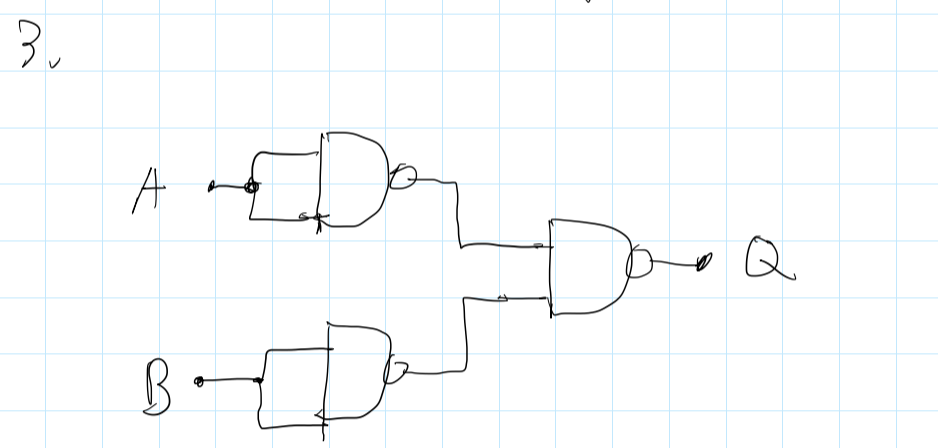
\includegraphics[width=0.7\textwidth]{./img/Lab 10/10_3_1.png}
        \caption{NANDS Gates to Construct OR Gate}
        \label{fig:or_gate}
    \end{figure}
   
   \subsection*{\textbf{Question 3 - Discussion}}
   The results confirmed that the configuration of NAND gates successfully produced an OR gate. The output followed the expected truth table for an OR gate, outputting 1 when either input was 1. This demonstrates that NAND gates can be used to create OR gates, providing flexibility in logic circuit design by combining basic components.
   
   \subsection*{\textbf{Procedure - Question 4}}
   For Question 4, we set up the CD4007 MOS transistor array, which contains six complementary MOS transistors (three N-channel and three P-channel FETs). This IC allowed us to configure the transistors to perform basic logic operations.
   
   \textbf{1. Component Identification:}
      - We identified the pins on the CD4007 corresponding to the N-channel and P-channel FETs, referring to Figure 2 in the lab manual for pin layout.
      \\
      - The N-channel FETs are used for low-side switching, and the P-channel FETs are used for high-side switching.
      \\
   
   \textbf{2. Setup:}
      - We configured the breadboard to prepare for the following exercises, ensuring that each transistor could be connected appropriately according to each circuit diagram.
      \\

    \subsection*{\textbf{Procedure - Question 5: Passive Pullup Inverter}}
    In Question 5, we built an inverter with a passive pullup resistor as shown in Figure 3.

    \begin{figure}[H]
        \centering
        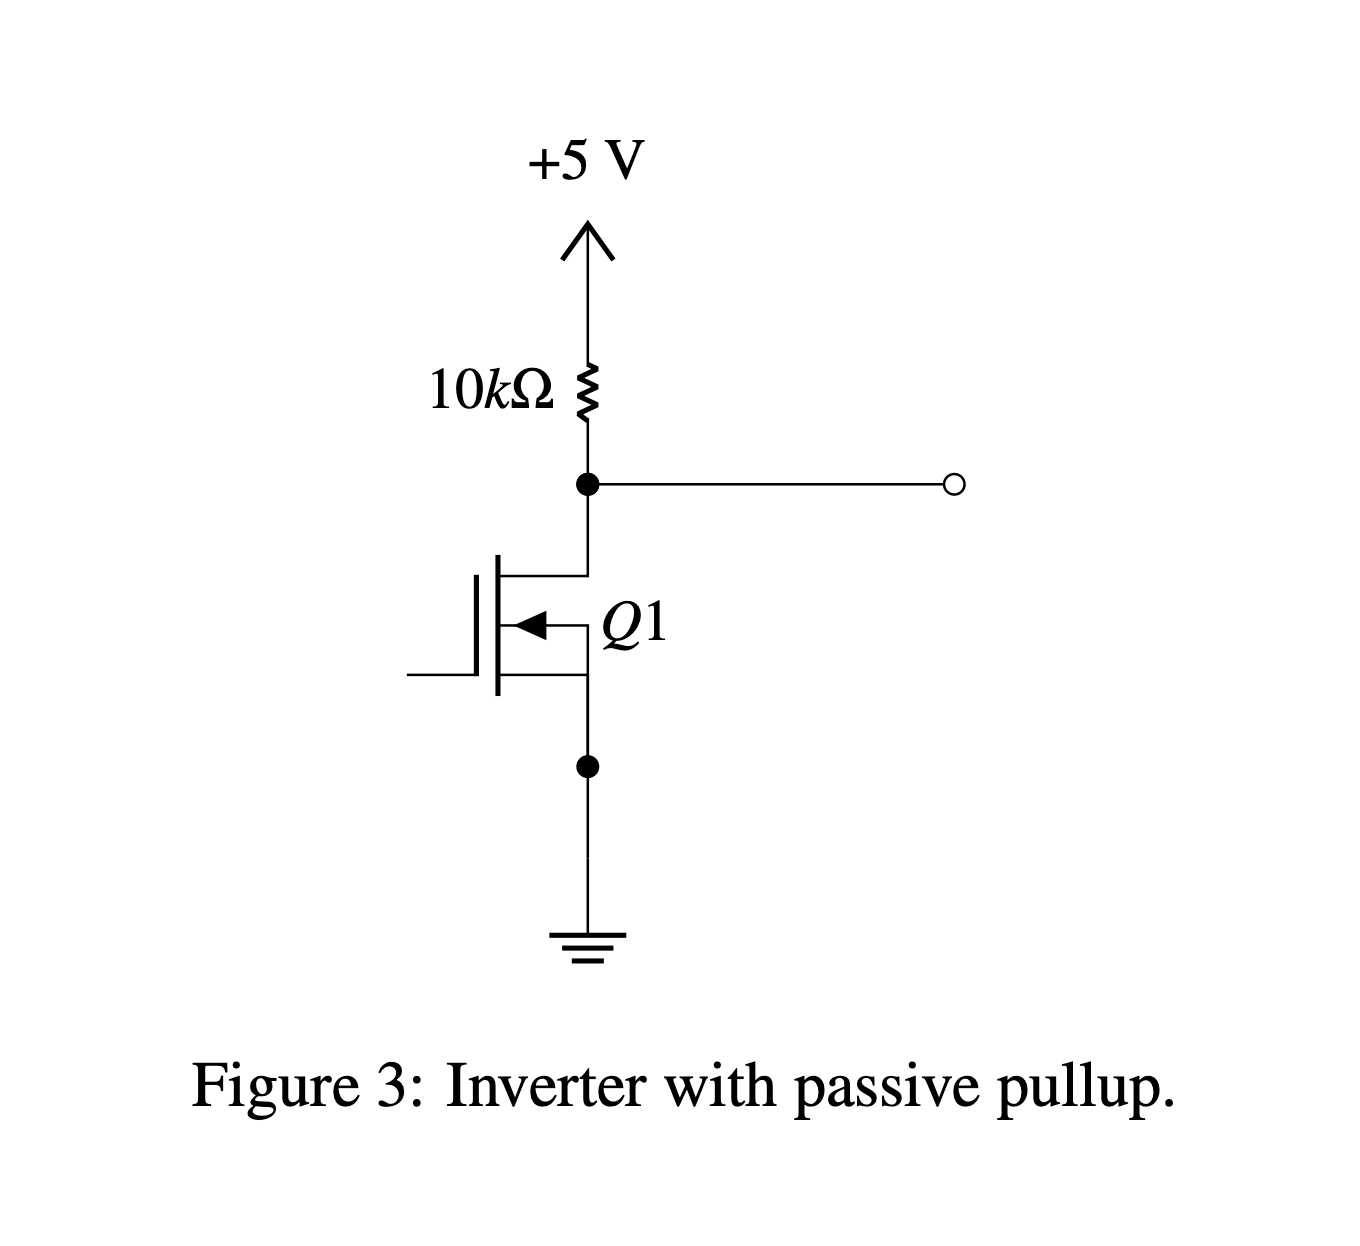
\includegraphics[width=0.7\textwidth]{./img/Lab 10/10_5_1.png}
        \caption{Passive Pullup Inverter Circuit}
        \label{fig:passive_pullup_inverter}
    \end{figure}

    \textbf{1. Circuit Construction:}
       - We connected the TTL output of the pulse generator to the input of the inverter.
       \\
       - A 1k resistor was used as a pullup, connecting the output to +5V.
       \\

    \textbf{2. Testing and Observations:}
       - We confirmed that the circuit inverted the input signal, outputting a low signal when the input was high and vice versa.
       \\
       - Next, we gradually increased the frequency of the input signal to determine the inverter’s behavior at higher frequencies.
       \\

    \subsection*{\textbf{Results - Question 5}}
    As we increased the frequency, we observed that the output started to degrade at high frequencies. The passive pullup could not fully charge or discharge the capacitance quickly enough, resulting in slower transitions and a less defined output.

    \subsection*{\textbf{Question 5 - Discussion}}
    The results indicate that while the passive pullup inverter performs adequately at lower frequencies, it suffers from significant degradation at higher frequencies. This is due to the time constant associated with the resistor and the inherent capacitance, which limits the circuit’s ability to respond to rapid changes in input.

    \subsection*{\textbf{Procedure - Question 6: Active Pullup Inverter}}
    In Question 6, we constructed an inverter using an active pullup configuration, as shown in Figure 4.

    \begin{figure}[H]
        \centering
        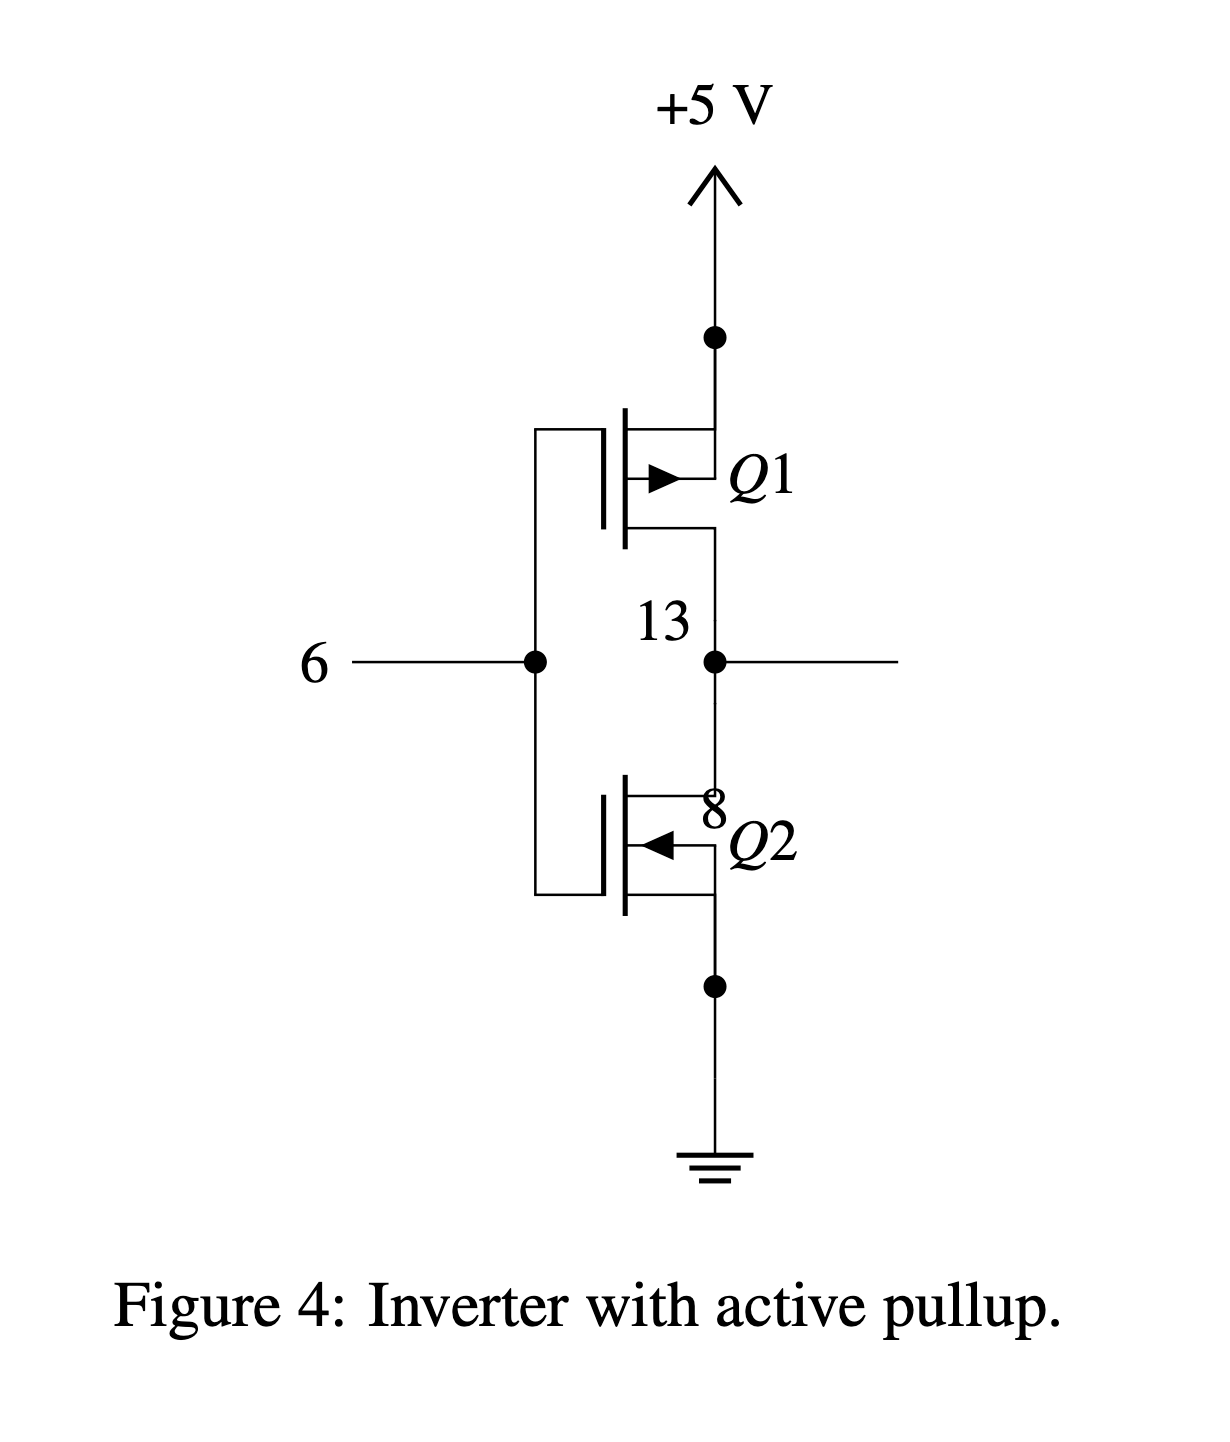
\includegraphics[width=0.7\textwidth]{./img/Lab 10/10_6_1.png}
        \caption{Passive Pullup Inverter Circuit}
        \label{fig:passive_pullup_inverter}
    \end{figure}

    \textbf{1. Circuit Construction:}
       - We used both an N-channel and a P-channel FET from the CD4007 to create an active pullup inverter.
       \\
       - The input signal was connected to both transistors, with the P-channel FET connected to +5V and the N-channel FET connected to ground.
       \\

    \textbf{2. Testing and Observations:}
       - We applied a TTL pulse from the generator to the input and observed the output on the oscilloscope.
       \\
       - As in the previous question, we increased the frequency of the input signal to observe any changes in behavior.
       \\

    \subsection*{\textbf{Results - Question 6}}
    The active pullup inverter demonstrated a more robust performance at higher frequencies compared to the passive pullup inverter. The output transitions were sharper and more consistent, with less signal degradation observed even as the input frequency increased significantly.

    \subsection*{\textbf{Question 6 - Discussion}}
    The active pullup inverter is more effective at handling high-frequency signals than the passive pullup configuration. The complementary configuration of N-channel and P-channel FETs allows for faster transitions, as each transistor actively pulls the output to the desired level, reducing the impact of capacitance.

    \subsection*{\textbf{Procedure - Question 7: NAND Gate Using CD4007 MOS Transistor Array}}
    In Question 7, we used the CD4007 MOS transistor array to construct a CMOS NAND gate using complementary MOSFETs. The CD4007 contains three N-channel and three P-channel MOSFETs, which can be configured to create various logic gates. We used two P-channel MOSFETs (for the pull-up network) and two N-channel MOSFETs (for the pull-down network) to form the NAND gate.
    
    \textbf{1. Pin Connections:}
    
    To replicate the CMOS NAND gate circuit, we used the following pin connections on the CD4007:
    
    \begin{itemize}
        \item \textbf{Vdd (Pin 14):} Connect this pin to the positive supply voltage (+5V). This supplies power to the P-channel MOSFETs.
        \item \textbf{GND (Pin 7):} Connect this pin to ground (0V), which serves as the ground for the N-channel MOSFETs.
        \item \textbf{Input A (Pin 6):} Connect this pin to the gate of both Q1 (P-channel) and Q3 (N-channel).
        \item \textbf{Input B (Pin 8):} Connect this pin to the gate of both Q2 (P-channel) and Q4 (N-channel).
        \item \textbf{Output (Pin 3):} This pin serves as the output of the NAND gate. It is the common connection between the drains of Q1 and Q2 (connected to Vdd) and the drains of Q3 and Q4 (connected to ground).
    \end{itemize}
    
    \begin{figure}[H]
        \centering
        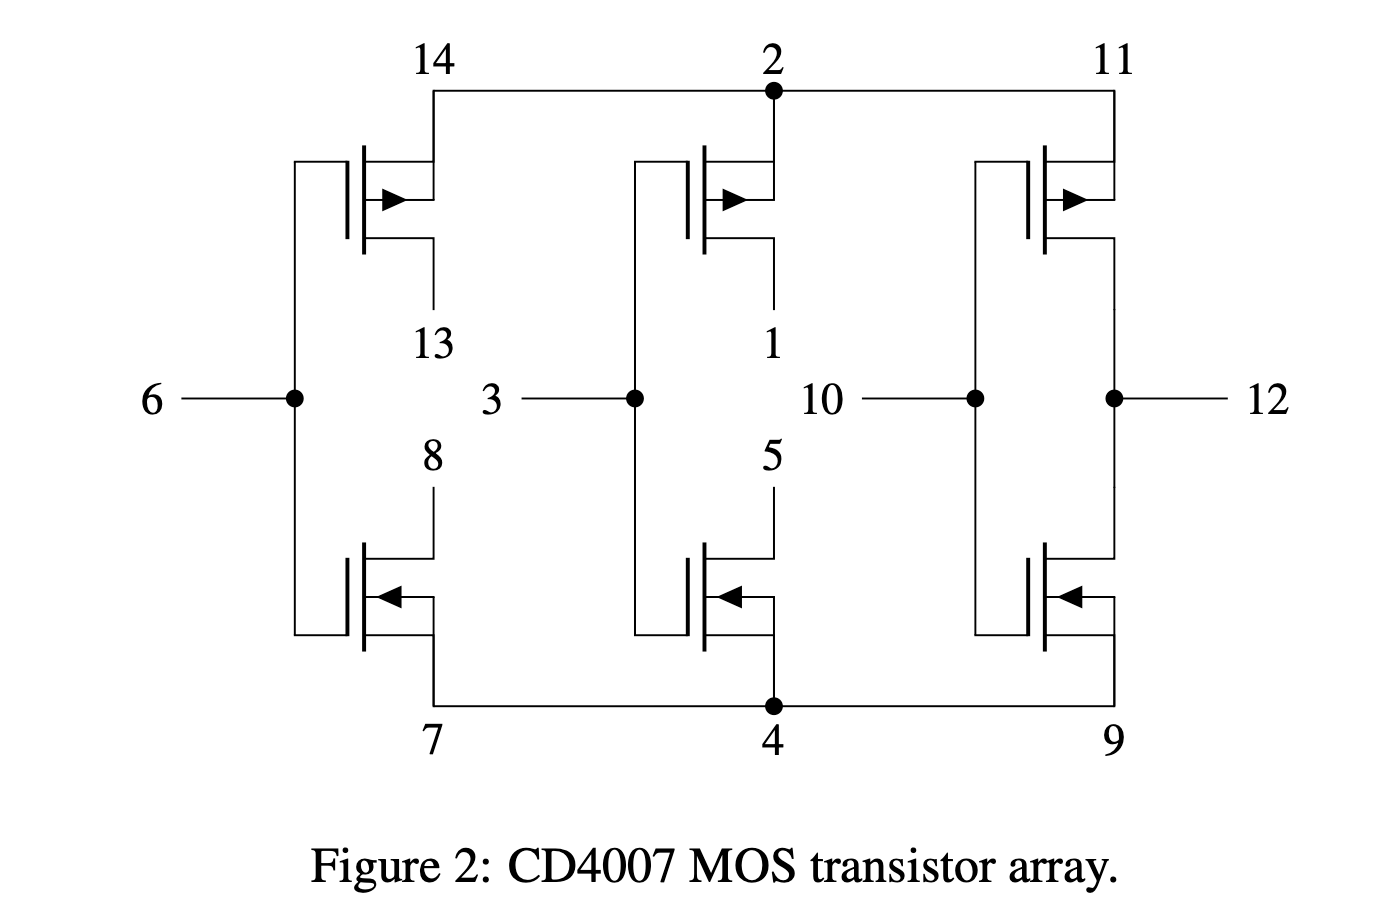
\includegraphics[width=0.5\textwidth]{./img/Lab 10/10_7_1.png} 
        \caption{CMOS NAND Gate using CD4007 MOS Transistor Array}
        \label{fig:CMOS_NAND_Gate}
    \end{figure}
    
    \textbf{2. Operation of the CMOS NAND Gate:}
    
    The following describes the operation of the NAND gate based on the input combinations:
    
    \begin{itemize}
        \item \textbf{Input A = 0, Input B = 0:} Q1 and Q2 (P-channel MOSFETs) are \textbf{ON}, connecting the output to Vdd, resulting in a high output (1).
        \item \textbf{Input A = 0, Input B = 1:} Q1 remains \textbf{ON}, and Q4 is \textbf{OFF}, keeping the output high (1) through Q1.
        \item \textbf{Input A = 1, Input B = 0:} Q2 remains \textbf{ON}, and Q3 is \textbf{OFF}, keeping the output high (1) through Q2.
        \item \textbf{Input A = 1, Input B = 1:} Both Q1 and Q2 (P-channel MOSFETs) are \textbf{OFF}, while Q3 and Q4 (N-channel MOSFETs) are \textbf{ON}, creating a path to ground and resulting in a low output (0).
    \end{itemize}
    
    \subsection*{\textbf{Results - Question 7}}
    The truth table below summarizes the operation of the CMOS NAND gate circuit:
    
    \begin{table}[H]
        \centering
        \caption{Truth Table for CMOS NAND Gate}
        \begin{tabular}{|c|c|c|}
            \hline
            Input A & Input B & Output \\
            \hline
            0 & 0 & 1 \\
            0 & 1 & 1 \\
            1 & 0 & 1 \\
            1 & 1 & 0 \\
            \hline
        \end{tabular}
    \end{table}
    
    \subsection*{\textbf{Question 7 - Discussion}}
    The CMOS NAND gate operates as expected based on the complementary configuration of the transistors: \\ 
    
       - When both inputs are low (0), the P-channel transistors Q1 and Q2 conduct, pulling the output high.
       \\
       - If either input is low, at least one P-channel transistor is on, maintaining a high output.
       \\
       - When both inputs are high (1), the N-channel transistors Q3 and Q4 conduct, connecting the output to ground and resulting in a low output.
       \\
    
    This configuration leverages the complementary action of P-channel and N-channel MOSFETs, which allows for efficient switching with minimal power consumption when idle. CMOS technology provides good noise margins and low power dissipation, making it ideal for digital logic circuits. This experiment demonstrates that the CD4007 can be effectively used to create basic logic gates like the NAND gate.




\section*{Lab 11: Digital Circuits II}

    \subsection*{Objective}
    The objective of Lab 11 was to explore sequential logic circuits by constructing basic flip-flop circuits using NAND gates. We verified the functionality of the R (Reset) and S (Set) inputs in a simple flip-flop configuration, and added clock control to the flip-flop to create a clocked sequential circuit.

    \subsection*{\textbf{Procedure - Question 1: Basic RS Flip-Flop}}
    In Question 1, we used two NAND gates from a single chip (either CMOS or TTL) to build the simplest example of a sequential logic circuit, an \textbf{RS flip-flop}. This circuit has two inputs: \textbf{S} (Set) and \textbf{R} (Reset). The outputs, labeled \textbf{Q} and \textbf{\(\overline{Q}\)}, hold their states even when the inputs are removed, demonstrating basic memory functionality.

    \textbf{1. Circuit Setup:}
    - We connected two NAND gates as shown in Figure 1. The output of the first NAND gate (IC1) is connected to one input of the second NAND gate (IC2), and vice versa, creating a feedback loop.
    \\
    - The \textbf{S} input is connected to the remaining input of IC1, while the \textbf{R} input is connected to the remaining input of IC2.
    \\
    - The \textbf{Q} output is taken from IC1, and the \textbf{\(\overline{Q}\)} output is taken from IC2.
    \\

    \begin{figure}[H]
        \centering
        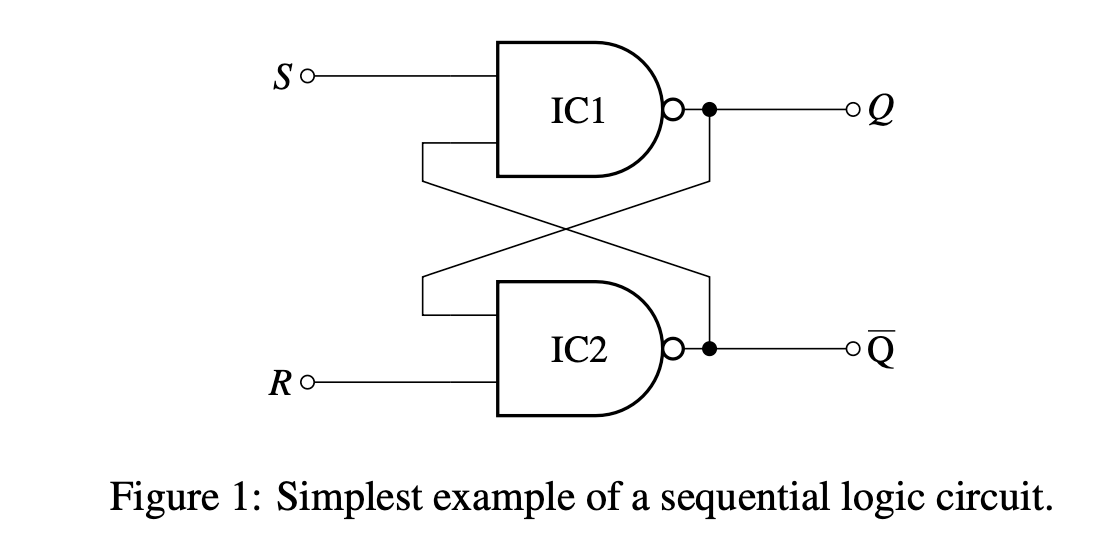
\includegraphics[width=0.5\textwidth]{./img/Lab 11/11_1_1.png} 
        \caption{RS Flip-Flop using two NAND gates}
        \label{fig:RS_FlipFlop}
    \end{figure}

    \textbf{2. Testing Procedure:}
    - We tested the circuit by applying different combinations of high (1) and low (0) signals to the \textbf{S} and \textbf{R} inputs.
    \\
    - For each combination, we observed and recorded the state of \textbf{Q} and \textbf{\(\overline{Q}\)}.
    \\

    \subsection*{\textbf{Results - Question 1}}
    The following table shows the expected output states for the RS flip-flop: \\

    \begin{table}[H]
        \centering
        \caption{Truth Table for RS Flip-Flop}
        \begin{tabular}{|c|c|c|c|}
            \hline
            S & R & Q & \(\overline{Q}\) \\
            \hline
            0 & 0 & Previous State & Previous State \\
            0 & 1 & 0 & 1 \\
            1 & 0 & 1 & 0 \\
            1 & 1 & Undefined & Undefined \\
            \hline
        \end{tabular}
    \end{table}

    \subsection*{\textbf{Discussion - Question 1}}
    The RS flip-flop operated as expected:
    - When \textbf{S = 1} and \textbf{R = 0}, the output \textbf{Q} is set to 1, and \textbf{\(\overline{Q}\)} is set to 0.
    \\
    - When \textbf{S = 0} and \textbf{R = 1}, the output \textbf{Q} is reset to 0, and \textbf{\(\overline{Q}\)} is set to 1.
    \\
    - When both \textbf{S} and \textbf{R} are 0, the flip-flop holds its previous state.
    \\
    - When both \textbf{S} and \textbf{R} are 1, the outputs are undefined, as this is an invalid state for an RS flip-flop.
    \\

    This basic configuration demonstrates how a flip-flop circuit can store information, maintaining its output state even when the inputs change back to 0.

    \subsection*{\textbf{Procedure - Question 2: Clocked RS Flip-Flop}}
    In Question 2, we extended the RS flip-flop circuit by adding two additional NAND gates to introduce clock control, resulting in a \textbf{clocked RS flip-flop}. The clock input determines when the state of the flip-flop can change, making it a more controlled sequential logic circuit.

    \textbf{1. Circuit Setup:}
    - We connected four NAND gates as shown in Figure 2. IC1 and IC2 are configured as in the previous RS flip-flop circuit, while IC3 and IC4 add the clock control.
    \\
    - The \textbf{S} and \textbf{R} inputs are connected to IC1 and IC2, respectively, while a clock input (active-low) is connected to the remaining inputs of IC1 and IC2.
    \\
    - The output \textbf{Q} is taken from IC3, and \textbf{\(\overline{Q}\)} is taken from IC4.
    \\

    \textbf{2. Testing Procedure:}
    - We applied different combinations of \textbf{S}, \textbf{R}, and \textbf{Clock} signals to verify the circuit’s behavior.
    \\
    - We observed whether the clock input effectively controlled the \textbf{Q} output, allowing it to change states only when the clock was active (low).
    \\

    \subsection*{\textbf{Results - Question 2}}
    The table below summarizes the expected output states for the clocked RS flip-flop: \\ 

    \begin{table}[H]
        \centering
        \caption{Truth Table for Clocked RS Flip-Flop}
        \begin{tabular}{|c|c|c|c|c|}
            \hline
            Clock & S & R & Q & \(\overline{Q}\) \\
            \hline
            0 & 0 & 0 & Previous State & Previous State \\
            0 & 0 & 1 & 0 & 1 \\
            0 & 1 & 0 & 1 & 0 \\
            1 & X & X & Previous State & Previous State \\
            \hline
        \end{tabular}
    \end{table}

    \subsection*{\textbf{Discussion - Question 2}}
    The clocked RS flip-flop successfully controlled the output based on the clock input: \\ 
    - When the clock was low, the circuit operated similarly to the basic RS flip-flop, allowing the \textbf{Q} output to be set or reset based on the \textbf{S} and \textbf{R} inputs.
    \\
    - When the clock was high, the flip-flop maintained its previous state, regardless of changes to \textbf{S} and \textbf{R}. This behavior illustrates the use of a clock input to control when the flip-flop can change states, which is essential in sequential circuits where timing is important.
    \\

    The addition of the clock input allows this circuit to function as a more controlled sequential logic element, only updating the output state when the clock is active. This setup is commonly used in digital systems where synchronization with a timing signal is necessary.

    \begin{figure}[H]
        \centering
        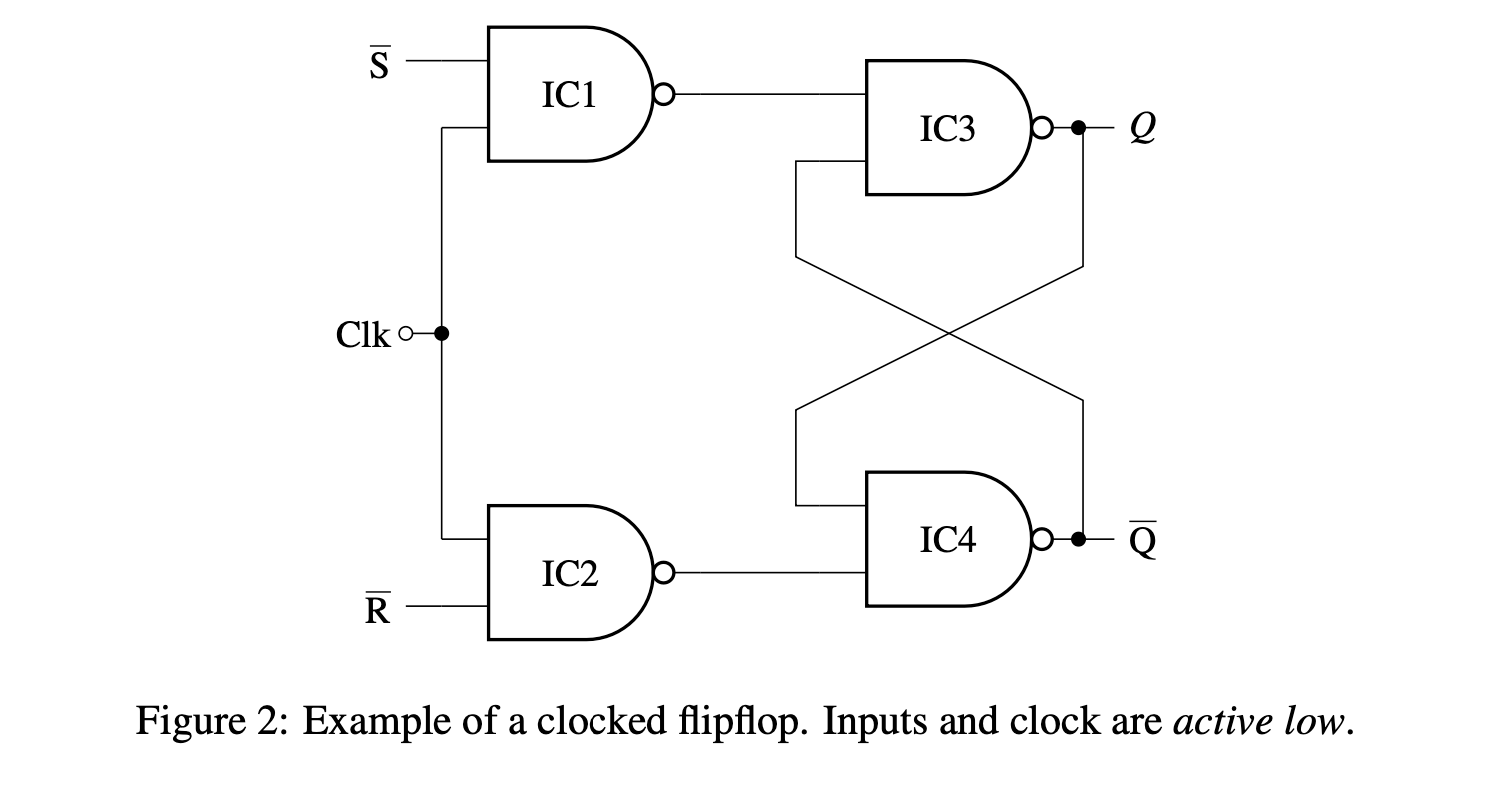
\includegraphics[width=0.5\textwidth]{./img/Lab 11/11_2_1.png}  % 
        \caption{Oscilloscope Trace for D Flip-Flop with Positive Edge-Triggered Clock}
        \label{fig:D_FlipFlop_Oscilloscope}
    \end{figure}
    
    \subsection*{\textbf{Procedure - Question 3: Initial Setup of the D Flip-Flop}}
    In Question 3, we used the SN74HCT74N D Flip-Flop, which includes two positive edge-triggered D flip-flops with SET (Preset) and RESET (Clear) inputs. We configured the circuit as follows:

    \textbf{1. Circuit Setup:} \\
    - We connected the \textbf{SET} (Preset) and \textbf{RESET} (Clear) pins to \textbf{high} (+5V) to disable them, ensuring that the flip-flop would respond only to the \textbf{D} and \textbf{Clock} inputs.
    \\
    - We used only one flip-flop from the SN74HCT74N, leaving the inputs of the second flip-flop tied to ground to avoid floating states.
    \\

    \textbf{2. Pin Connections:} \\ 
    - \textbf{D input (Pin 2):} Connected to a slide switch to control the data input.
    \\
    - \textbf{Clock input (Pin 3):} Connected to a debounced pushbutton switch, allowing us to manually control the clock pulses.
    \\
    - \textbf{Q output (Pin 5)} and \(\overline{\textbf{Q}}\) output (Pin 6): Observed on the oscilloscope to monitor the flip-flop’s response.
    \\

    \subsection*{\textbf{Procedure - Question 4: Testing the D Flip-Flop Operation}}
    In Question 4, we tested the D Flip-Flop by: \\
    - Setting the D input using the slide switch.
    \\
    - Triggering the clock input using the pushbutton switch to produce a positive edge.
    \\
    - Observing the behavior of the Q output on the oscilloscope, verifying that the Q output followed the D input only when the clock transitioned from low to high (positive edge-triggered).
    \\

    \textbf{Expected Behavior:} \\ 
    - When the clock input receives a rising edge (0 to 1 transition), the Q output takes on the value of the D input.
    \\
    - If the D input is high (1) at the clock’s rising edge, Q will be set to high (1). If the D input is low (0), Q will be set to low (0).
    \\
    - Between clock pulses, the Q output holds its state, providing a memory function.
    \\
    - Activating the SET (Preset) or RESET (Clear) inputs would override the D and Clock inputs, forcing Q to 1 or 0, respectively, but these inputs were held high in this experiment.
    \\

    \begin{figure}[H]
        \centering
        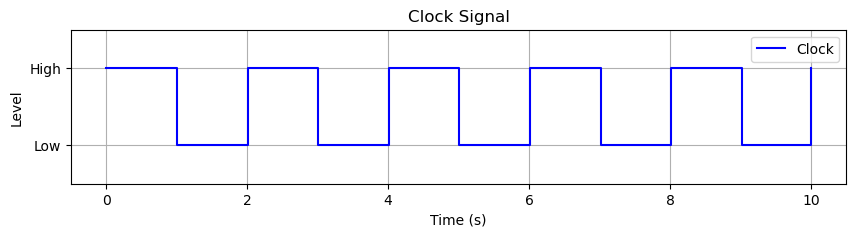
\includegraphics[width=0.8\textwidth]{./img/Lab 11/11_3_1.png}  % 
        \caption{Oscilloscope Trace for D Flip-Flop with Positive Edge-Triggered Clock, Clock Trace}
        \label{fig:D_FlipFlop_Oscilloscope_1}
    \end{figure}

    \begin{figure}[H]
        \centering
        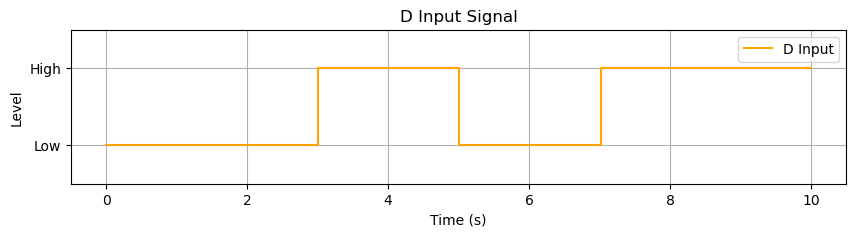
\includegraphics[width=0.8\textwidth]{./img/Lab 11/11_3_2.png}  % 
        \caption{Oscilloscope Trace for D Flip-Flop with Positive Edge-Triggered Clock, D Input Trace}
        \label{fig:D_FlipFlop_Oscilloscope_2}
    \end{figure}

    \begin{figure}[H]
        \centering
        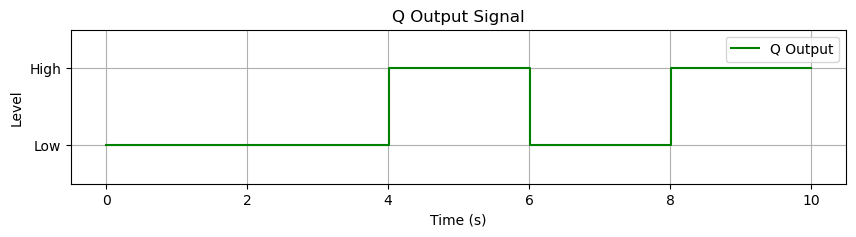
\includegraphics[width=0.8\textwidth]{./img/Lab 11/11_3_3.png}  % 
        \caption{Oscilloscope Trace for D Flip-Flop with Positive Edge-Triggered Clock, Q Output Trace}
        \label{fig:D_FlipFlop_Oscilloscope_3}
    \end{figure}

    \subsection*{\textbf{Results - Questions 3 and 4}}
    The table below summarizes the expected behavior of the D Flip-Flop based on the D and Clock inputs:

    \begin{table}[H]
        \centering
        \caption{Expected Behavior of Positive Edge-Triggered D Flip-Flop}
        \begin{tabular}{|c|c|c|c|}
            \hline
            D Input & Clock (Rising Edge) & Q Output & \(\overline{Q}\) Output \\
            \hline
            0 & ↑ & 0 & 1 \\
            1 & ↑ & 1 & 0 \\
            X & 0 & Previous State & Complement of Q \\
            \hline
        \end{tabular}
    \end{table}

    \subsection*{\textbf{Discussion - Questions 3 and 4}}
    The SN74HCT74N D Flip-Flop responded as expected: \\ 
    - The Q output only changed state on the rising edge of the clock, assuming the value of the D input at that moment.
    \\
    - Between clock pulses, the Q output maintained its previous state, illustrating the memory behavior of the flip-flop.
    \\
    - This setup demonstrates the utility of a D Flip-Flop for storing a bit of information that updates only in response to a clock signal, a fundamental function in digital circuits.
    \\

    The oscilloscope trace (Figure \ref{fig:D_FlipFlop_Oscilloscope_1} - \ref{fig:D_FlipFlop_Oscilloscope_3}) shows the timing relationship between the Clock, D input, and Q output, confirming the edge-triggered behavior of the flip-flop.

    
    \subsection*{\textbf{Procedure - Question 5: D Flip-Flop with Feedback}}
    In Question 5, we connected the Q output of the D Flip-Flop (SN74HCT74N) back to its D input, creating a feedback loop as shown in Figure 4. This configuration allows the circuit to toggle its state on each clock pulse.
    
    \textbf{1. Circuit Setup:} \\ 
       - The \textbf{SET} (Preset) and \textbf{RESET} (Clear) inputs were tied to \textbf{high} (+5V) to disable them. \\
       - The \textbf{D input (Pin 2)} was connected to the \textbf{Q output (Pin 5)} through a feedback wire. \\
       - The \textbf{Clock input (Pin 3)} was connected to either a debounced pushbutton for manual control or a function generator for automatic clocking. \\
       - The outputs, \textbf{Q (Pin 5)} and \textbf{\(\overline{Q}\) (Pin 6)}, were monitored on the oscilloscope. \\
    
    \textbf{2. Testing Procedure:} \\
       - Initially, the clock input was manually toggled using the pushbutton, and the Q output was observed to verify the toggling behavior. \\ 
       - The clock input was then connected to a function generator, and the Q output was observed at increasing clock frequencies. The propagation delay was measured as the time difference between the rising edge of the clock and the change in the Q output. \\
    
    \begin{figure}[H]
        \centering
        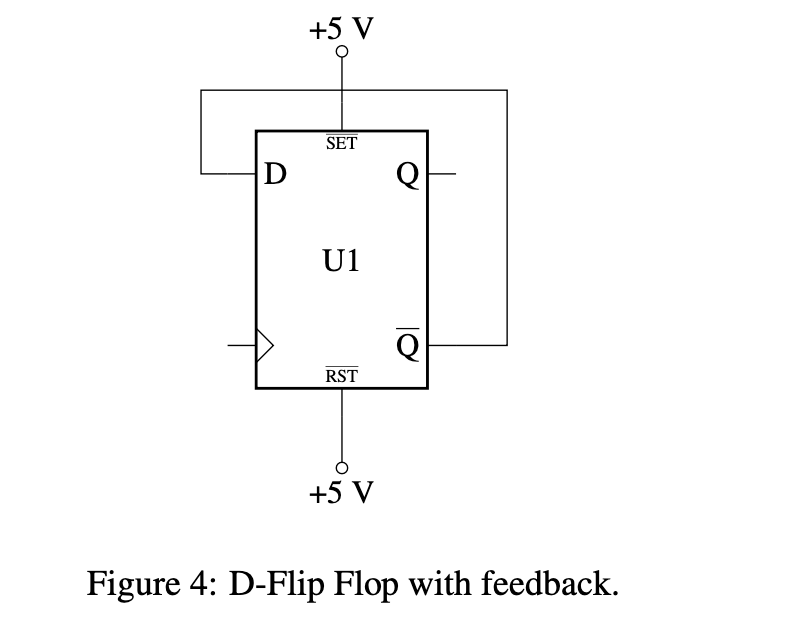
\includegraphics[width=0.5\textwidth]{./img/Lab 11/11_5_1.png}  
        \caption{D Flip-Flop with Feedback Connection}
        \label{fig:Feedback_Circuit}
    \end{figure}
    
    \subsection*{\textbf{Results - Question 5}}
    The expected behavior of the D Flip-Flop with feedback is as follows: \\ 
       - On each rising edge of the clock, the Q output toggles between 0 and 1. \\
       - At higher clock frequencies, the propagation delay becomes more apparent, with the Q output transitioning slightly after the clock’s rising edge. \\ 
    
    \begin{figure}[H]
        \centering
        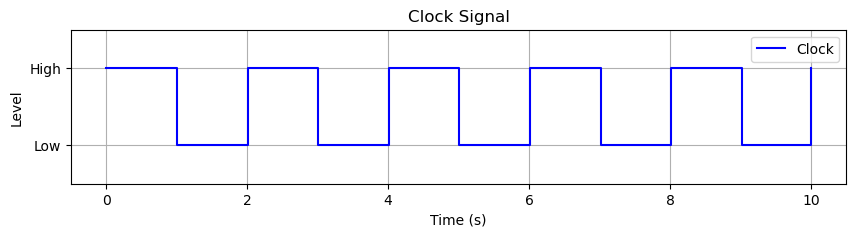
\includegraphics[width=0.8\textwidth]{./img/Lab 11/11_5_2.png}  
        \caption{Clock Signal for D Flip-Flop with Feedback}
        \label{fig:Clock_Signal_Feedback}
    \end{figure}
    
    \begin{figure}[H]
        \centering
        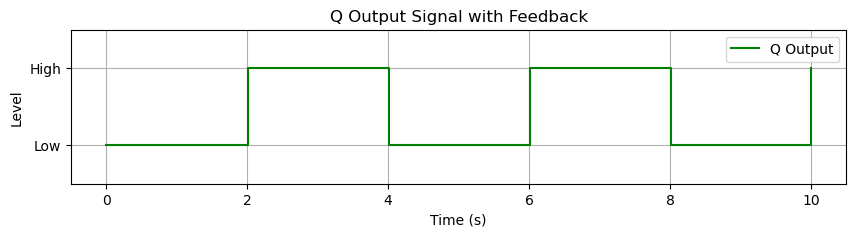
\includegraphics[width=0.8\textwidth]{./img/Lab 11/11_5_3.png}  %
        \caption{Q Output Signal with Feedback for D Flip-Flop}
        \label{fig:Q_Output_Feedback}
    \end{figure}
    
    \subsection*{\textbf{Discussion - Question 5}}
    The D Flip-Flop with feedback demonstrates the ability to toggle its state on each clock pulse: \\ 
       - \textbf{Manual Clocking:} The Q output alternated between 0 and 1 with each press of the pushbutton. \\
       - \textbf{Function Generator Clocking:} The circuit continued to toggle with each clock pulse. At higher clock frequencies, the propagation delay became evident, as the Q output lagged slightly behind the clock rising edge. \\
    
    \textbf{Graph Analysis:} \\
       - The \textbf{Clock Signal (Figure 16)} shows the timing control of the circuit, with rising edges indicating the moments where the flip-flop evaluates its inputs. \\
       - The \textbf{Q Output Signal (Figure 17)} demonstrates toggling behavior, where the output alternates between high and low on each clock rising edge. This is due to the feedback loop that connects the Q output to the D input. \\ 
       - Compared to earlier graphs, the Q output no longer depends on an external D input but autonomously toggles based on the feedback mechanism. \\
    
    \textbf{Relevance of Propagation Delay:} \\
       - The propagation delay is the time between the rising edge of the Clock signal and the change in the Q output. This delay is critical in high-speed digital systems, as it determines the maximum operating frequency of the circuit. \\
       - In this setup, the propagation delay becomes evident at higher clock frequencies, where the Q output may fail to toggle if the clock period is shorter than the delay. \\
    
    This question illustrates the utility of feedback in creating toggle flip-flops, which are fundamental building blocks in counters and sequential digital logic circuits.
    

    \subsection*{\textbf{Procedure - Question 6: Cascaded D Flip-Flops}}
    In Question 6, we cascaded two D Flip-Flops (U1 and U2) as shown in Figure 5. The Q output of the first flip-flop (U1) was connected to the Clock input of the second flip-flop (U2), forming a Ripple Counter.

    \textbf{1. Circuit Setup:} \\
    - Both flip-flops were part of the same SN74HCT74N IC, each with its \textbf{SET} and \textbf{RESET} inputs tied high (+5V) to disable them. \\
    - The Clock input for the first flip-flop (U1) was driven by a function generator. \\
    - The Q output of U1 was connected to the Clock input of the second flip-flop (U2). \\
    - The D inputs of both flip-flops were connected to their respective Q outputs via feedback loops, ensuring toggling behavior. \\

    \begin{figure}[H]
        \centering
        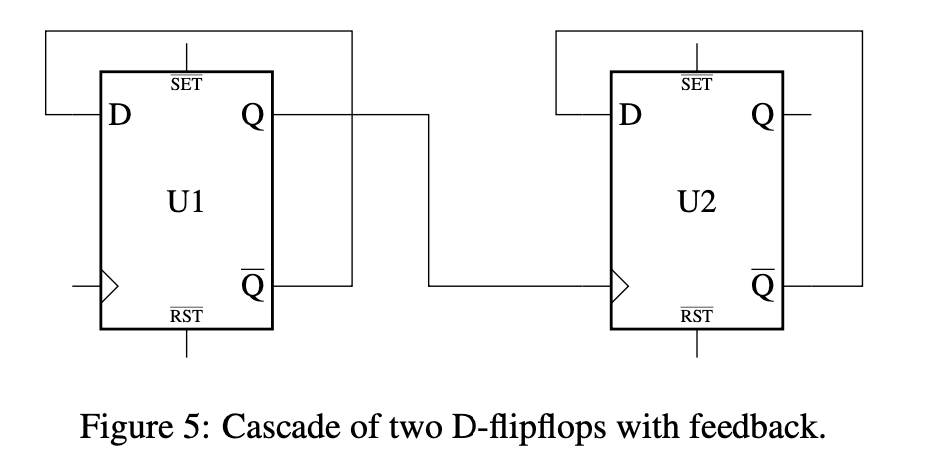
\includegraphics[width=0.6\textwidth]{./img/Lab 11/11_6_1.png} 
        \caption{Cascaded D Flip-Flops with Feedback}
        \label{fig:Cascaded_FlipFlops}
    \end{figure}

    \textbf{2. Testing Procedure:} \\
    - The Clock signal for U1 was varied using a function generator, and the Q outputs of U1 and U2 were observed on the oscilloscope. \\
    - The frequency of the Clock signal was increased to observe the behavior of the cascaded flip-flops at higher frequencies. \\

    \subsection*{\textbf{Results - Question 6}}
    The following behavior was observed: \\
    - U1 toggled its Q output on every rising edge of the Clock signal, just as in Question 5. \\
    - U2 toggled its Q output on every rising edge of U1’s Q output, effectively dividing the frequency of the Clock signal by 4. \\

    \begin{figure}[H]
        \centering
        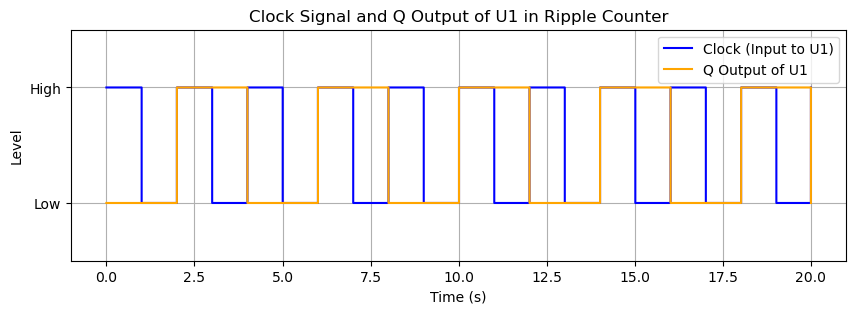
\includegraphics[width=0.8\textwidth]{./img/Lab 11/11_6_2.png}  
        \caption{Clock Signal and Q Output of U1 in Ripple Counter}
        \label{fig:Clock_U1_Ripple}
    \end{figure}

    \begin{figure}[H]
        \centering
        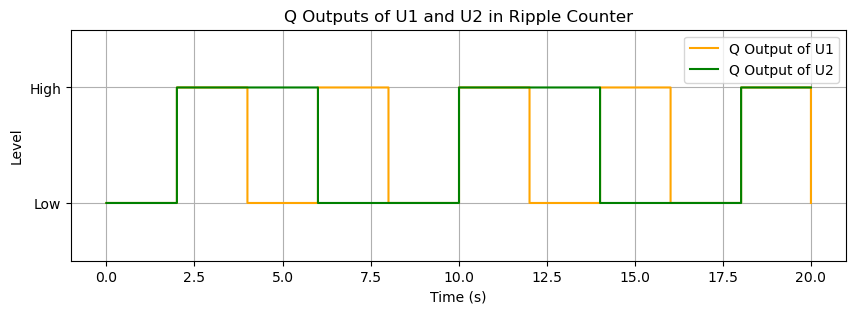
\includegraphics[width=0.8\textwidth]{./img/Lab 11/11_6_3.png} 
        \caption{Q Outputs of U1 and U2 in Ripple Counter}
        \label{fig:Q_Outputs_Ripple}
    \end{figure}

    \subsection*{\textbf{Discussion - Question 6}}
    The Ripple Counter demonstrates how cascading D Flip-Flops can divide a clock frequency: \\
    - The Q output of U1 acts as the Clock input for U2, effectively dividing the frequency of the original Clock signal. \\
    - As a result, U1 toggles at half the frequency of the original Clock, and U2 toggles at half the frequency of U1, resulting in a division by 4 overall. \\

    \textbf{Comparison to Previous Questions:} \\
    - In Question 5, we observed a single flip-flop toggling on each clock pulse, creating a frequency division of 2. Cascading two flip-flops extends this concept to divide the frequency further. \\
    - The timing diagrams show a clear progression: \\
        - The Clock signal determines the toggling behavior of U1 (as in Question 5). \\
        - U2 toggles at a lower frequency, emphasizing the cumulative delay introduced by cascading. \\

    \textbf{Graph Analysis:} \\
    - \textbf{Figure \ref{fig:Clock_U1_Ripple}:} Shows the Clock signal for U1 and its Q output, verifying the toggle behavior at half the clock frequency. \\
    - \textbf{Figure \ref{fig:Q_Outputs_Ripple}:} Demonstrates the sequential toggling of U1 and U2, with U2 toggling at a frequency that is one-fourth of the original Clock signal. \\

    The cascaded configuration highlights how propagation delays and sequential toggling behavior can be exploited to create frequency dividers and counters. This fundamental concept is widely used in digital design for timekeeping, division, and state counting.

    \subsection*{\textbf{Estimated Behavior - Questions 7 and 8}}
    \\
    \textbf{Question 7: Cascading Four Flip-Flops with LEDs}
    Since we didn't have enough time to 

    In this configuration, the Q outputs of four flip-flops (U1, U2, U3, and U4) are connected to four LEDs. The LEDs represent a binary counter:

    \textbf{Behavior:} \\
    - Each flip-flop toggles at half the frequency of the previous one. \\
    - The four LEDs display a binary counting sequence, progressing through states such as 0000, 0001, 0010, and so on. \\

    \textbf{Interpretation of Output:} \\
    - The LEDs visually represent the state of a 4-bit binary counter. \\
    - This configuration demonstrates the cascading effect of flip-flops and their application in digital counting circuits. \\

    \\
    \textbf{Question 8: Shift Register with Four Flip-Flops}

    The shift register shifts data sequentially across the four flip-flops: \\ 

    \textbf{Clock and Input Behavior:} \\ 
    - The clock signal synchronizes the timing of data shifts. \\ 
    - Data at the IN input is propagated through the flip-flops, appearing on the Q outputs of U1, U2, U3, and U4 sequentially. \\

    \textbf{Expected Oscilloscope Observations:} \\
    - The IN signal appears as a series of pulses, representing the data to be shifted. \\
    - The Q outputs show the progression of this data through the register, with a one-clock-cycle delay for each flip-flop. \\

    \textbf{Jitter Explanation:} \\
    - Jitter, caused by propagation delays or noise, results in minor timing discrepancies between clock edges and data transitions. \\
    - While not significant at low frequencies, jitter becomes more pronounced in high-speed systems. \\

    This experiment showcases the practical applications of cascaded and sequential flip-flop configurations in digital systems.

    


  
\end{document}
